\section{Inversion}

In order to flip a matrix upside down, we first had to generate an identity matrix of the appropriate size where the rows had the opposite diagonal direction.

    \[
      \underbrace{
        \begin{bmatrix}
          1&0&0\\
          0&1&0\\
          0&0&1\\
        \end{bmatrix}
      }_{\text{Identity Matrix}}
      \implies
      \underbrace{
        \begin{bmatrix}
          0&0&1\\
          0&1&0\\
          1&0&0\\
        \end{bmatrix}
      }_{\text{Transformation Matrix}}
    \]

This was done by setting up the identity matrix as a two dimensional array; in other words, a list of lists. Then this list was iterated through and each list in the main list was flipped front-to-back. This action had the same effect as flipping the entire matrix on the horizontal axis. Finally, as before with the shifting process, we multiplied the matrix on the appropriate side of the matrix.

    \[
      \begin{bmatrix}
        0&0&1\\
        0&1&0\\
        1&0&0\\
      \end{bmatrix}
      \cdot
      \begin{bmatrix}
        a&b&c\\
        d&e&f\\
        g&h&i\\
      \end{bmatrix}
      =
      \underbrace{
      \begin{bmatrix}
        g&h&i\\
        d&e&f\\
        a&b&c\\
      \end{bmatrix}
      }_{\text{The inverted
      matrix}}
    \]

This resulted in images that were upside down, as is demonstrated in figure \eqref{fig:flipped}

    \begin{figure}[h!]
        \centering
        \begin{subfigure}{0.6\textwidth}
            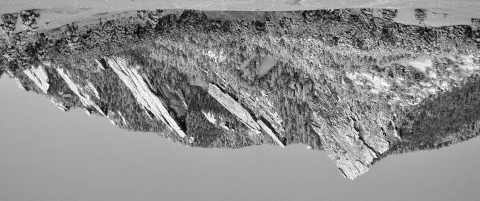
\includegraphics[scale=0.5]{./img/flip1.png}
            \caption{Image 1 Flipped}
        \end{subfigure}
        \begin{subfigure}{0.3\textwidth}
            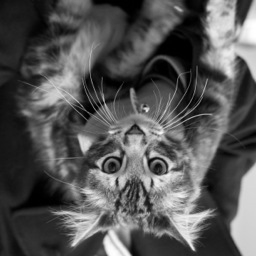
\includegraphics[scale=0.5]{./img/flip2.png}
            \caption{Image 2 Flipped}
        \end{subfigure}
        \caption{Our Flipped Images}
        \label{fig:flipped}
    \end{figure}


The Python code to flip images is below.

        \lstinputlisting[language=Python,
                        showstringspaces=false,
                        frame=single,
                        firstline=102,
                        lastline=111,
                        basicstyle=\ttfamily,
                        keywordstyle=\color{blue},
                        numbers=left,
                        commentstyle=\color{red}]{./py/analysis.py}
